\begin{center}
	\Huge
	Residualer og residualanalyse
\end{center}

\section*{Residualer}
\stepcounter{section}

Vi forestiller os at have observeret følgende $n$ punkter \\ $(x_1,y_1),(x_2,y_2),\hdots,(x_n,y_n)$ samt en model $f$, der beskriver datasættet. Så kan det ofte være meningsfuldt at have et mål for, hvor godt modellen rent faktisk beskriver observationssættet. Til dette er \textit{residualerne} for modellen et af de mest hyppigt anvendte redskaber. Disse defineres på følgende vis.
\begin{defn}[Residualer]
	For et datasæt $(x_1,y_1),(x_2,y_2),\hdots,(x_n,y_n)$ samt en model $f$ defineres det $i$'te residual
	$r_i$ som
	\begin{align*}
		r_i = y_i - f(x_i).
	\end{align*}
\end{defn}
På Figur \ref{fig:residual} kan vi se en illustration af residualerne for en model $f$.
\begin{figure}[H]
	\centering
	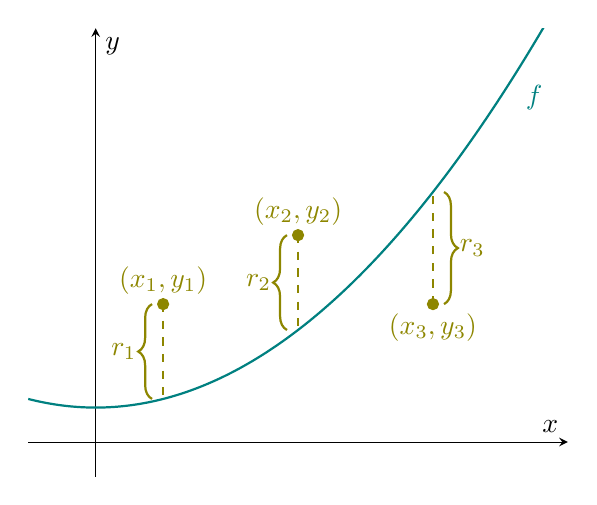
\begin{tikzpicture}
	\begin{axis}[
	axis lines = center,
	ticks = none, 
	xlabel = $x$, ylabel = $y$, 
	xmin = -1, xmax = 7,
	ymin = -1, ymax = 12,
	]
		\node[color = teal] at (axis cs: 6.5,10) {$f$}; 
		\addplot[color = teal, thick, domain = -1:7, samples = 200] {0.25*x^2 + 1}; 
		\filldraw[color = olive] (axis cs: 1,4) circle (2pt) node[anchor = south] {$(x_1,y_1)$};
		\filldraw[color = olive] (axis cs: 3,6) circle (2pt) node[anchor = south] {$(x_2,y_2)$};
		\filldraw[color = olive] (axis cs: 5,4) circle (2pt) node[anchor = north] {$(x_3,y_3)$};
		\draw[color = olive, dashed, thick] (axis cs: 1,4) -- (axis cs: 1,1.25);
		\draw[decorate,decoration={brace,amplitude=5pt,mirror,raise=4pt}, color = olive, thick ]
			(axis cs: 1, 4) -- (axis cs: 1, 1.25) node[midway, anchor = east, xshift = -6pt] {$r_1$}; 	
		\draw[color = olive, dashed, thick] (axis cs: 3,6) -- (axis cs: 3,3.25);
		\draw[decorate,decoration={brace,amplitude=5pt,mirror,raise=4pt}, color = olive, thick ]
			(axis cs: 3, 6) -- (axis cs: 3, 3.25) node[midway, anchor = east, xshift = -6pt] {$r_2$};
		\draw[color = olive, dashed, thick] (axis cs: 5,4) -- (axis cs: 5,7.25);
		\draw[decorate,decoration={brace,amplitude=5pt,mirror,raise=4pt}, color = olive, thick ]
			(axis cs: 5, 4) -- (axis cs: 5, 7.25) node[midway, anchor = west, xshift = 6pt] {$r_3$};
	\end{axis}	
	\end{tikzpicture}
	\caption{Tre residualer visualiseret for punkterne $(x_1,y_1)$, $(x_2,y_2)$ og $(x_3,y_3)$ samt modellen $f$.}
	\label{fig:residual}
\end{figure}
\begin{exa}
	Vi betragter tilfældet, hvor vi har observeret datasættet $(2,5)$, $(3,6)$ og $(5,4)$. Vi bruger modellen 
	$f$ givet ved
	\begin{align*}
		f(x) = \frac{1}{2}x^2 - 1
	\end{align*}
	til at beskrive datasættet. Anvender vi definitionen for residualerne på disse punkter, så får vi følgende 
	residualer.
	\begin{align*}
		r_1 &= 5 - f(2) = 5 - 1 = 4, \\
		r_2 &= 6 - f(3) = 6 - 3.5 = 2.5, \\
		r_3 &= 4 - f(5) = 4 - 11.5 = -7.5.
	\end{align*}
	Man kan overveje, hvad dette siger om modellen. Er det godt eller dårligt? Og hvordan afgør vi, om en anden 
	model er bedre?
\end{exa}


\section*{Residualanalyse}
\stepcounter{section}
For at afgøre, om et sæt af residualer for en model er godt eller dårligt, kan vi anvende forskellige former for residualanalyse. Vi skal i dag arbejde med en mere kvalitativ vurdering af et sæt residualer, og ofte vil
en vurdering af residualer både i forskning og industrien være af kvalitativ karakter. 

Vi tager udgangspunkt i et eksempel.

\begin{exa}
Vi betragter datapunkterne fra \href{https://github.com/ChristianJLex/TeachingNotes/raw/master/2023-2024/Data og lign/regression_eksempel.xlsx}{\color{blue!60} dette datasæt}.
Vi ved ikke, hvilken underlæggende sammenhæng, der skaber dataet, kan vi prøve at lave forskellige regressioner på det. Dette gøres i Maple og kan ses af Figur \ref{fig:regression}.

\begin{figure}[H]
\centering
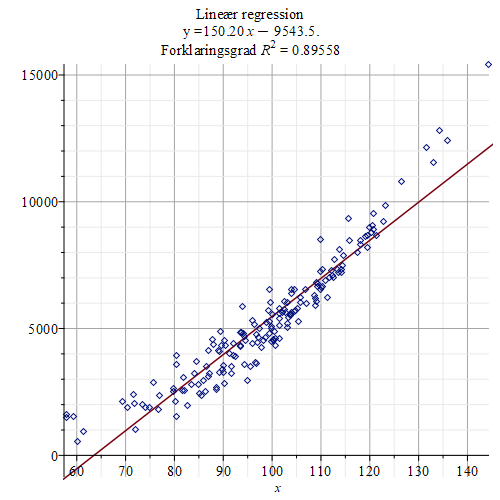
\includegraphics[width = \textwidth*4/10]{Billeder/LinRegtilRes.png}
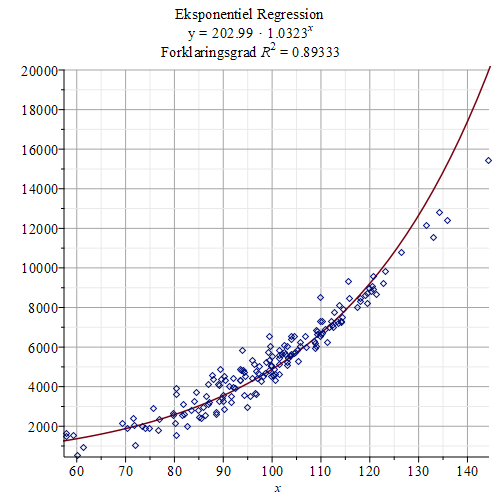
\includegraphics[width = \textwidth*4/10]{Billeder/ExpRegtilRes.png}
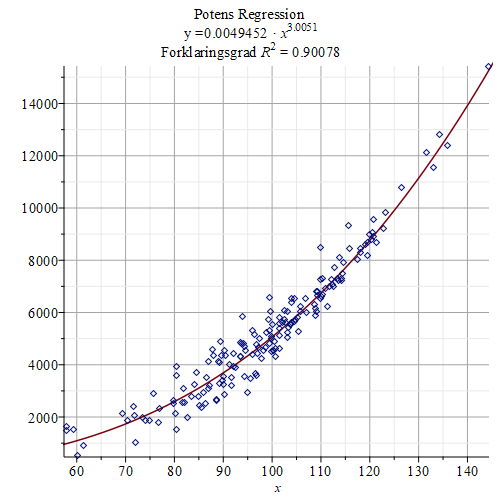
\includegraphics[width = \textwidth*4/10]{Billeder/PowRegtilRes.png}
\caption{Lineær regression, eksponentiel regression og potensregression på datasæt}
\label{fig:regression}
\end{figure}
Hvordan afgør vi så, hvilken af modellerne der er bedst, hvis vi ikke har yderligere information omkring kilden af dataet? Man kan ikke sammenligne korrelationskoefficienter mellem modeller. Derfor skal vi lave regressionsanalyse. En del af regressionsanalyse er blot at betragte de fittede modeller og se, hvilken model der ser ud til at passe bedst. I dette tilfælde ser det ud til at være potensmodellen. 
\end{exa}


Det er klart, at en god model $f(x)$ vil have små residualer. Udover dette så vil vi også have normalfordelte residualer. Det vil sige, at vi gerne vil have mange residualer tæt på 0 og kun få langt fra 0. Der må ikke være nogen yderligere struktur i residualerne. For at se, hvad dette betyder, ser vi på et eksempel.

\begin{exa}
Betragter vi regressionerne fra tidligere eksempel, kan vi finde residualerne for de tre modeller. Disse findes i Maple ved eksempelvis
\begin{align*}
	\texttt{plotResidualer(X,Y,LinReg)} 
\end{align*}
 i fald residualerne skal findes for lineær regression. Residualerne for de tre modeller kan ses af Fig. \ref{fig:resplot}
\begin{figure}[H]
\centering
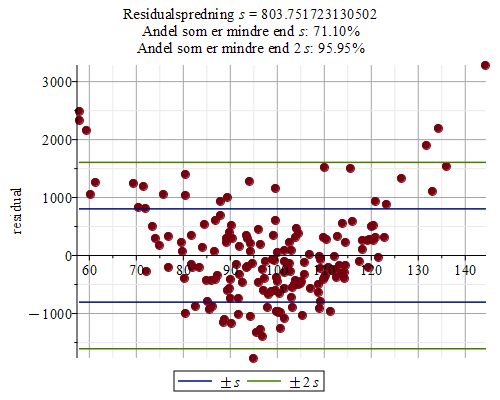
\includegraphics[width = \textwidth*4/10]{Billeder/LinRegResidual.png}
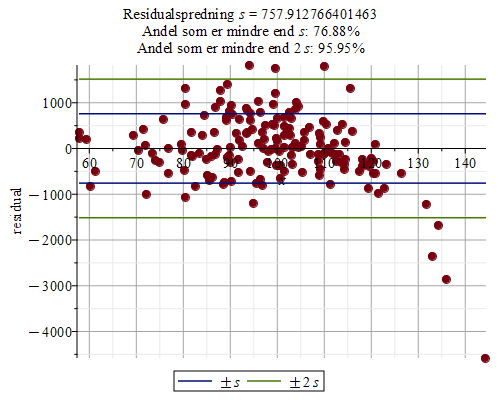
\includegraphics[width = \textwidth*4/10]{Billeder/ExpRegResidual.png}
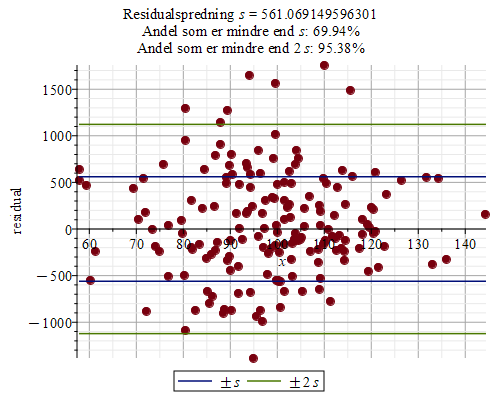
\includegraphics[width = \textwidth*4/10]{Billeder/PowRegResidual.png}
\caption{Lineær regression, eksponentiel regression og potensregression på datasæt}
\label{fig:resplot}
\end{figure}
	Vi ønsker at se et tilfældigt mønster i residualerne, og derfor ser det ud til at 
	potensregressionen beskriver datapunkterne bedst.
\end{exa}

\section*{Polynomiel regression}
\stepcounter{section}

Nøjagtigt som vi har set det med lineære, eksponentielle og potensfunktioner kan vi også lave
\textit{polynomiel regression}. Har vi et datasæt, vi antager kan beskrives af et polynomium af grad $n$, så kan vi lave polynomiel regression i Maple ved kommandoen
\begin{align*}
	&\texttt{restart} \\
	&\texttt{with(Gym):} \\
	&\texttt{PolyReg(data,n)} 
\end{align*}
hvor \texttt{data} er vores datasæt. 
\begin{exa}
	Vi får givet \href{https://github.com/ChristianJLex/TeachingNotes/raw/master/2023-2024/Data og lign/poly_example.xlsx}{\color{blue!60} dette datasæt} og forventer, at det kan beskrives af 
	et tredjegradspolynomium. Vi importerer det til Maple og laver polynomiel regression ved at 
	skrive
	\begin{align*}
		&\texttt{restart}\\
		&\texttt{with(Gym):}\\
		&\texttt{PolyReg(data,3)}
	\end{align*}
	Resultatet af dette kan ses af Figur \ref{fig:polyreg}.
	\begin{figure}[H]
		\centering
		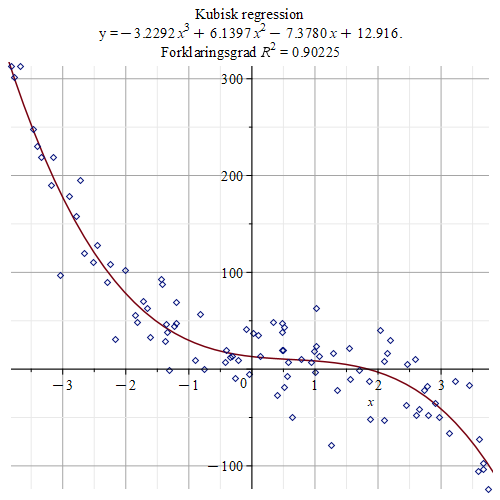
\includegraphics[width=0.7\textwidth]{Billeder/polyreg2}
		\caption{Polynomiel regression af 3. grad}
		\label{fig:polyreg}
	\end{figure}
	Hvis vi er interesserede i, hvor godt polynomiet beskriver datasættet, kan vi anvende 
	residualplottet. Dette får vi frem ved i Maple at skrive
	\begin{align*}
		\texttt{plotResidualer(data,[PolyReg,3])}
	\end{align*}
	Plottet kan ses af Figur \ref{fig:polyresidual}.
	\begin{figure}[H]
		\centering
		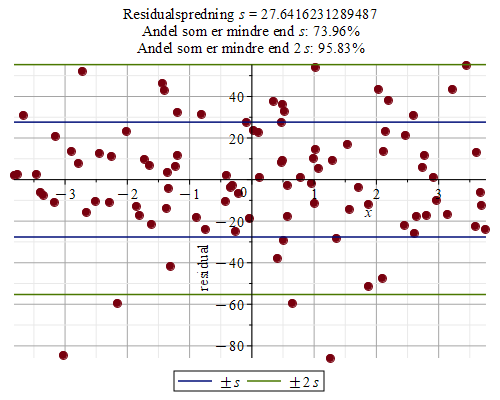
\includegraphics[width=0.7\textwidth]{Billeder/polyresidual}
		\caption{Residualplot for polynomiel regression}
		\label{fig:polyresidual}
	\end{figure}
	Af Figur \ref{fig:polyresidual} kan vi se, at residualerne ser tilfældigt spredte ud. 
	Derfor tror vi på, at modellen beskriver datasættet godt. 
\end{exa}
Det er vigtigt at bemærke, at vi altid skal vælge den polynomiumsmodel, der har lavest grad og som ser ud til at beskrive datasættet godt. Dette skal vi gøre, da vi i princippet kan beskrive datasættet vilkårligt godt med en høj nok polynomiel grad, men dette gør, at vi mister den underliggende sammenhæng mellem $x$- og $y$-værdierne. 



\subsection*{Opgave 1}
Et datasæt er givet ved $(2,10)$, $(5,7)$, $(7,-1)$ og $(10,-5)$ og en model $f$ er givet ved
\begin{align*}
	f(x) = -3x + 15.
\end{align*}
\begin{enumerate}[label=\roman*)]
	\item Bestem residualerne $r_1$, $r_2$, $r_3$ og $r_4$ for modellen. 
\end{enumerate}

\subsection*{Opgave 2}
Et datasæt $(2,y_1)$, $(4,y_2)$ og $(6,y_3)$ har residualerne $r_1 = -1$, $r_2 = 4$ og $r_3 = 7$ for modellen
\begin{align*}
	f(x) = x^2 -2x + 1.
\end{align*}
\begin{enumerate}[label=\roman*)]
	\item Bestem de observerede værdier $y_1$, $y_2$ og $y_3$.
\end{enumerate}



\subsection*{Opgave 3 (med hjælpemidler)}
\stepcounter{section}

Et datasæt er givet ved følgende tabel
\begin{center}
\begin{tabular}{c|c|c|c|c|c|c|c|c|c}
1 & 2 & 3 & 4 & 5 & 6 & 7 & 8 & 9 & 10\\ \hline
1.45 & 14.96 & 7.22 & 26.63 & 45.49 & 66.88 & 103.90&157.63 & 162.63 & 252.61
\end{tabular}
\end{center}

\begin{enumerate}[label=\roman*)]
	\item Afgør, hvilken regressionsmodel, der passer bedst.
	\item Bestem residualet $r_5$. 
\end{enumerate}

\subsection*{Opgave 4 (med hjælpemidler)}

I \href{https://github.com/ChristianJLex/TeachingNotes/raw/master/2023-2024/Data%20og%20lign/bakterierResidual.xlsx}{\color{blue!60} dette datasæt} findes antal bakterier i mia. sammenholdt med den forløbne tid i timer i en bestemt bakteriekoloni. 

\begin{enumerate}[label=\roman*)]
	\item Afgør, hvilken regressionstype, der passer bedst på datasættet ved at bruge 
	residualerne for modellen.
	\item Brug din valgte model til at bestemme, hvor mange bakterier der vil være efter 30 
	timer.
	\item Bestem residualet til tidspunktet 7 timer. 
\end{enumerate}

\subsection*{Opgave 5 (med hjælpemidler)}

I \href{https://github.com/ChristianJLex/TeachingNotes/raw/master/2023-2024/Data%20og%20lign/beboereResidual.xlsx}{\color{blue!60} dette datasæt} findes antal beboere i en by angivet efter antal forløbne år efter år 1900.

\begin{enumerate}[label=\roman*)]
	\item Afgør, hvilken regressionstype, der passer bedst på datasættet ved at bruge 
	residualerne for modellen.
	\item I hvilket år vil der i følge din model være 8000 beboere i byen?
\end{enumerate}

\subsection*{Opgave 6 (med hjælpemidler)}

I \href{https://github.com/ChristianJLex/TeachingNotes/raw/master/2023-2024/Data og lign/Baevervaegt.xlsx}{\color{blue!60} dette datasæt} fremgår længden i cm og vægten i kg af 122 europæiske bævere. 

\begin{enumerate}[label=\roman*)]
	\item Afgør, hvilken regressionstype, der passer bedst på datasættet ved at bruge 
	residualerne for modellen.
	\item Hvor lang skal en bæver ifølge modellen være for at veje 25kg?
\end{enumerate}

\subsection*{Opgave 7 (med hjælpemidler)}

I \href{https://github.com/ChristianJLex/TeachingNotes/raw/master/2023-2024/Data og lign/Chokoladepris.xlsx}{\color{blue!60} dette datasæt} fremgår sammenhængen mellem prisen på en bestem plade chokolade og antal passerede år efter år 1990.

\begin{enumerate}[label=\roman*)]
	\item Afgør, hvilken regressionstype, der passer bedst på datasættet ved at bruge 
	residualerne for modellen.
	\item Hvad er prisen på en plade chokolade i år 2010 ifølge modellen?
\end{enumerate}

\subsection*{Opgave 8 (med hjælpemidler)}

I \href{https://github.com/ChristianJLex/TeachingNotes/raw/master/2023-2024/Data og lign/Laegemiddel.xlsx}{\color{blue!60} dette datasæt} fremgår koncentrationen i blodet (i mg/L) af et bestemt lægemiddel og antal forløbne timer efter indtagelsen.

\begin{enumerate}[label=\roman*)]
	\item Afgør, hvilken regressionstype, der passer bedst på datasættet ved at bruge 
	residualerne for modellen.
	\item Hvornår er koncentrationen i blodet under 0.5mg/L?
\end{enumerate}

\subsection*{Opgave 9 (med hjælpemidler)}
	Et datasæt er givet \href{https://github.com/ChristianJLex/TeachingNotes/raw/master/2023-2024/Data og lign/poly_opgave1.xlsx}{\color{blue!60} her}.
	\begin{enumerate}[label=\roman*)]
		\item Brug residualplots til at bestemme den mindste polynomielle grads regression, 
		der beskriver datasættet godt. 
		\item Lav polynomiel regression med den grad, du har bestemt i i) og bestem 
		forskriften for det polynomium, der beskriver datasættet.
		\item Brug forskriften til at bestemme $f(4)$.
		\item Brug Maple til at finde rødderne for $f$.
	\end{enumerate}
\subsection*{Opgave 10 (med hjælpemidler)}
	Et datasæt er givet \href{https://github.com/ChristianJLex/TeachingNotes/raw/master/2023-2024/Data og lign/poly_opgave2.xlsx}{\color{blue!60} her}.
	\begin{enumerate}[label=\roman*)]
		\item Brug residualplots til at bestemme den mindste polynomielle grads regression, 
		der beskriver datasættet godt. 
		\item Lav polynomiel regression med den grad, du har bestemt i i) og bestem 
		forskriften for det polynomium $g$, der beskriver datasættet.
		\item Brug forskriften til at bestemme løsningen til ligningen $g(x)=12$
		\item Brug Maple til at finde rødderne for $g$.
	\end{enumerate}
	
\subsection*{Opgave 11 (med hjælpemidler)}
	Et datasæt er givet \href{https://github.com/ChristianJLex/TeachingNotes/raw/master/2023-2024/Data og lign/poly_opgave3.xlsx}{\color{blue!60} her}.
	\begin{enumerate}[label=\roman*)]
		\item Brug residualplots til at bestemme den mindste polynomielle grads regression, 
		der beskriver datasættet godt. 
		\item Lav polynomiel regression med den grad, du har bestemt i i) og bestem 
		forskriften for det polynomium $h$, der beskriver datasættet.
		\item Brug Maple til at finde rødderne for $h$.
	\end{enumerate}

\subsection*{Opgave 12 (med hjælpemidler)}
	Et datasæt er givet \href{https://github.com/ChristianJLex/TeachingNotes/raw/master/2023-2024/Data og lign/poly_opgave4.xlsx}{\color{blue!60} her}.
	\begin{enumerate}[label=\roman*)]
		\item Brug residualplots til at bestemme den mindste polynomielle grads regression, 
		der beskriver datasættet godt. 
		\item Lav polynomiel regression med den grad, du har bestemt i i) og bestem 
		forskriften for det polynomium $p$, der beskriver datasættet.
		\item Bestem skæringspunkterne mellem $p$ og $h$
	\end{enumerate}
	
\subsection*{Opgave 13 (med hjælpemidler)}
	Et datasæt er givet \href{https://github.com/ChristianJLex/TeachingNotes/raw/master/2023-2024/Data og lign/poly_opgave5.xlsx}{\color{blue!60} her}.
	\begin{enumerate}[label=\roman*)]
		\item Brug residualplots til at bestemme den mindste polynomielle grads regression, 
		der beskriver datasættet godt. 
		\item Lav polynomiel regression med den grad, du har bestemt i i) og bestem 
		forskriften for det polynomium $q$, der beskriver datasættet.
		\item Tegn $q$ på intervallet $[-10,10]$. Har $q$ et maksimum eller minimum på dette interval?
	\end{enumerate}

\subsection*{Opgave 14 (med hjælpemidler)}
	Et datasæt er givet \href{https://github.com/ChristianJLex/TeachingNotes/raw/master/2023-2024/Data og lign/poly_opgave6.xlsx}{\color{blue!60} her}.
	\begin{enumerate}[label=\roman*)]
		\item Brug residualplots til at bestemme den mindste polynomielle grads regression, 
		der beskriver datasættet godt. 
		\item Lav polynomiel regression med den grad, du har bestemt i i) og bestem 
		forskriften for det polynomium $r$, der beskriver datasættet.
		\item Løs ligningen $r(x) + p(x) = q(x)$.
	\end{enumerate}
